\chapter{Statistics}

\section {Probability Overview}
\subsection {Parameters Describing Distributions}
Mean and Median represent the \textbf{central tendency} of a distribution. \textbf{Mean} is essentially the center of gravity of a distribution: If we consider the values that a random variable takes as distances on a plank and their probabilities as weights, then the mean point would be the distance point on the plank below which, if a fulcrum is placed, the plank will be perfectly balanced. Hence the formula of mean $\mu$ is derived as below:
	\begin{align*}
		\int_{-\infty}^{\mu} (\mu-x)f_X(x)dx &= \int_{\mu}^{\infty} (x-\mu)f_X(x)dx \\
		\intertext{Since $\mu$ is a constant, we can pull it out of the integrals on both sides,} 
		\mu \int_{-\infty}^{\mu}f_X(x)dx - \int_{-\infty}^{\mu} xf_X(x)dx &= \int_{\mu}^{\infty} xf_X(x)dx - \mu \int_{\mu}^{\infty}f_X(x)dx \\
		\intertext{Rearranging the equation, we get,} 
		\mu \int_{-\infty}^{\mu}f_X(x)dx + \mu \int_{\mu}^{\infty}f_X(x)dx &= \int_{-\infty}^{\mu} xf_X(x)dx + \int_{\mu}^{\infty} xf_X(x)dx \\
		\mu \int_{-\infty}^{\infty}f_X(x)dx &= \int_{-\infty}^{\infty} xf_X(x)dx \\
		\intertext{Recognizing that the area under the probability curve for entire range of $x$ values is $1$,} 
		\mu &=  \int_{-\infty}^{\infty} xf_X(x)dx
	\end{align*}
Note that the above equation is only for continuous random variables which take real values from $-\infty$ to $\infty$. For all other cases, the formula and the derivation are similar. 

\textbf{Median} represents the midpoint value of the random variable, X, if the values of $X$ are ordered. It is the value, above and below which, there are equal \emph{number} of $X$ values. In other words, while mean is the central tendency if both $X$ values and their probabilities, median is the central tendency if only the probabilities are considered. Median is a more useful parameter in some contexts: Take, for instance, the wealth distribution among the people of India. Since most wealth is accumulated in the hands of a very small number of people, if one were to calculate the mean wealth it will be pulled in one direction due to the few people who have enormous wealth and hence may paint a rosy picture about the economic condition of the population in general. However, median wealth would inform that half the population is below that value and half the people have more wealth than that. So median would be a better indication of the economic condition of the population. 

Apart from Mean and Median, \textbf{Mode} is also an important parameter related to the ``signal part'' of a random variable (Explained in the next paragraph). It is simply the value of $X$ that occurs most frequently. Mode is more important than Mean or Median is some contexts: For ex., when we use the colloquial term, ``Average Indian'', we actually (technically) are talking about the Modal Indian. Because, with ``Average Indian'', we are talking about the ``Common Man'' that we are mostly likely to encounter in the streets. The ``Common Man'' has a certain income level, certain age, height, weight etc. If one thinks of a common man as a value the multi-dimensional random variable ``Indian'' can take, then the Mean value of that random variable would represent have the mean values of every dimension, i.e., income level, age etc., and that may be far away from the ``Common Man''. In fact, the ``Mean Indian'' may be a completely unrealistic person. But a ``Modal Indian'' is simply the multi-dimensional value of $X$ that occurs most frequently and, hence, by definition, a realistic person. 

Variance ($\sigma^2$) and, it's square root Standard Deviation ($\sigma$) represent the \textbf{spread} in the population. \textbf{Variance} is defined as $E[(X-\mu)^2]$. It is a common practice, while making measurements of a quantity, to take multiple measurements and then average out the resulting values. This is done because in most measurement instruments have tolerances defined as some $\pm k\%$ - If the error in the measurement (i.e., noise) has equal probability of taking slightly higher or lower values as compared to the true value (i.e., signal), then taking an average would zero out the noise. Hence, if we think of the measured value as a random variable, then mean would be the true value of a measurement and Variance, the probablistic version of the mean square error in the measurement. We need \textbf{Standard Deviation} because Variance is a square value and hence has squared units (ex. $km^2$) as compared to the measured quantity (ex. $km$) - Taking the square root of the mean square error gives us an error quantity with comparable units to the signal (Think of Signal-to-Noise ratio). This is why the Standard Deviation is also called the \textbf{standard error}.

Skewness and Kurtosis represent the \textbf{shape} of a distribution. \textbf{Skewness} ($\gamma_1$)of a dsitribution, defined as \( E[(\frac{X-\mu}{\sigma})^3] \), is the measure of asymmetry. A perfectly symmetric distribution has Skewness equal to $0$. Skewness will have a positive value if a random variable has higher probability of having low values. Skewness will have a positive value if a random variable has higher probability of having high values. Skewness is also called ``Pearson Skewness''.
	\begin{figure}
	  \centering
	    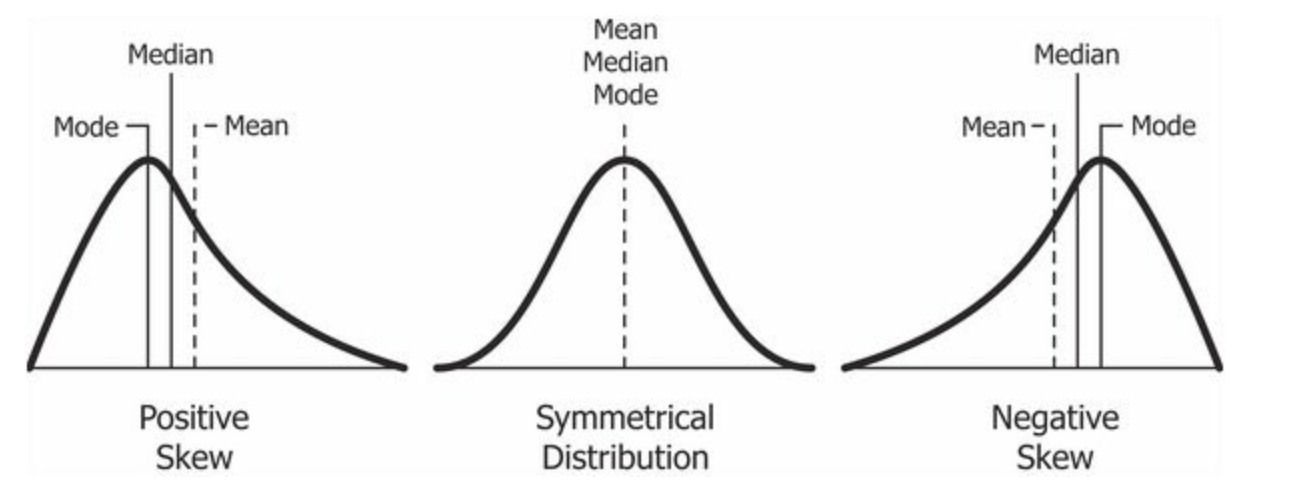
\includegraphics[width=\textwidth]{Statistics/Relationship_between_mean_and_median_under_different_skewness}
	  \caption{Relationships between different parameters}
	  \label{fig:parameter_interrelationship}
	\end{figure}

Figure \ref{fig:parameter_interrelationship} shows the relationship between skewness, mean, median and mode. Remember how we talked about how a few wealthy Indians could pull the mean and give a false story about the economic status of the population? The positively skewed (skewness is a positive value) distribution in the picture represents such a scenario: A lot of people (represented by y-axis) have low values (concentrated on the left side of the x-axis). 

\textbf{Kurtosis} ($\gamma_2$), is defined as \( E[(\frac{X-\mu}{\sigma})^4] \), is a measure of the peakedness or flatness of a distribution as compared to normal distribution (refer to Central Limit Theorem). Univariate Normal distribution has a Kurtosis of 3. If a distribution looks ``pulled up'' version of a normal distribution, its Kurtosis will be greater than 3, and if it looks ``stretched out'', the Kurtosis will be less than 3. Kurtosis is also called ``Pearson Kurtosis''

Note that, for a Normal distribution, Mean = Median = Mode, and Skewness is $0$, all of which establish a convenient baseline with which to compare other distributions (abNormal!). But Kurtosis alone, for a Normal distribution is 3! So, some people use an ``Adjusted Pearson Kurtosis'', which is simply $Kurtosis - 3$. In literature, if we find mentioning of ``Postive'' or ``Negative'' Kurtosis, it means they are talking about the Adjusted Pearson Kurtosis. In other contexts, one should be careful to find out whether a piece of literature uses Pearson Kurtosis or the adjusted version before interpreting the text.
	\begin{figure}
	  \centering
	    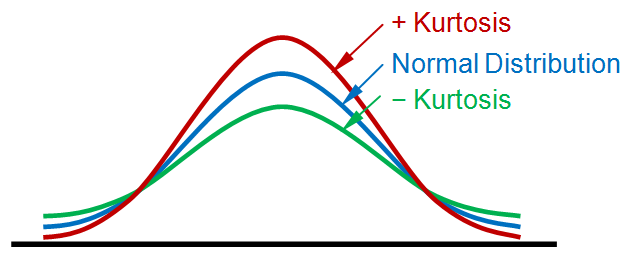
\includegraphics[width=\textwidth]{Statistics/kurtosis}
	  \caption{Adjusted Pearson Kurtosis}
	  \label{fig:kurtosis}
	\end{figure}

Figure \ref{fig:kurtosis} shows what positive and negetive (Adjusted Peason) Kurtosis looks like when compared with the normal distribution.  

So far, we have talked about parameters related to univariate distributions, where one random variable $X$ has a certain probability distribution associated with it. But sometimes a probability distribution is associated with a set of two random variables. Ex: We can associate probabilities to (height, weight) tuples for all the girls of a certain age. For such cases, some new parameters arise. \textbf{Covariance} ($\sigma_{XY}$), defined as \( Cov[X,Y] = E[(X-\mu_X)(Y-\mu_Y)] \). The usefulness of Covariance is apparent when you look at its normalized variant, namely the \textbf{Correlation Coefficient} ($\rho$), defined as \( \rho_{XY} = \frac{\sigma_{XY}}{\sigma_X \sigma_Y}\). The values of the Correlation Coefficient can vary from -1 to 1. When $X$ and $Y$ are independent, $\sigma_{XY}$ will be 0 and hence $\rho_{XY}$ will also be 0. If $Y$ is linearly dependent on $X$, then $\rho_{XY}$ will be 1 or -1. If $Y$ is loosely dependent on $X$, then $\rho$ values will be close to zero (on the positive or negative side). 
	\begin{figure}
	  \centering
	    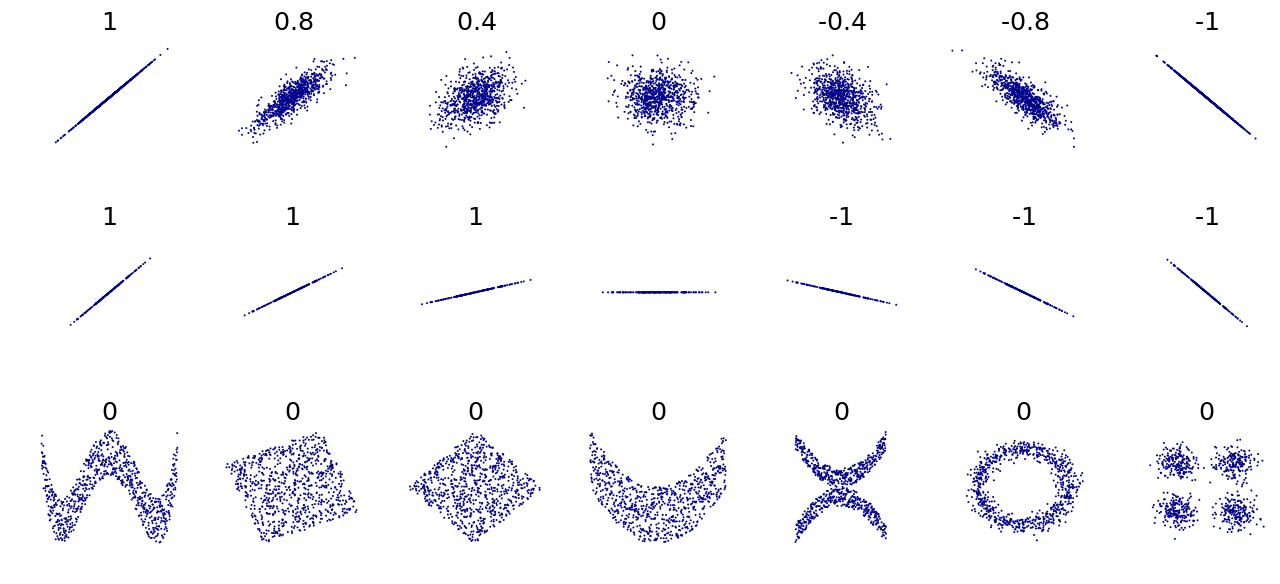
\includegraphics[width=\textwidth]{Statistics/correlation}
	  \caption{Correlation Coefficient of Various Joint Distributions}
	  \label{fig:correlation}
	\end{figure}

Figure \ref{fig:correlation} shows the graphical representation of distribution of (X,Y) tuples and the correlation coefficients in each case. One can see how the Correlation Coefficient gives an idea about the tightness and direction of the relationship between $X$ and $Y$.

\subsection {Common Probability Distributions}
The most basic distribution is the \textbf{Bernoulli distribution}. The Bernoulli random variable (R.V.) takes two values, 1/0 corresponding to Yes/No, On/Off etc. Coin flips, Gender of a person, bit error, Yes/No answers to survey questions etc., can be modeled as Bernoulli R.V.s. It has only one parameter $p$, the probability of getting a $1$ - knowing $p$, one can derive the only other unknown required to entirely describe the Bernoulli distribution, namely the probability of getting a $0$, because it is simply $1-p$, which is sometimes referred to as $q$\footnote{When a researcher models a survey question with a Yes/No answer, while looking at its statistical analysis, one should not automatically assume that ``Yes'' is considered $1$ and ``No'' is considered $0$. Same thing goes for gender. One should always check how the researcher has assigned R.V. values to the two possibilities. If you are the researcher, it is important to explicitly mention how you have done the assignment}. Most distributions of interest in probability theory and in statistics arise as extensions of Bernoulli distribution or closely associated with it. The following paragraphs talk about these distributions.

One can generalize a Bernoulli distribution to a case where the result can take a certain number of fixed values. This distribution is called a \textbf{Categorical distribution}. A six sided die, the colour of a candy coated chocolate etc., follow Categorical distributions. A Catergorical distribution is defined by $K-1$ parameters, where $K$ is the number of possible values the R.V. can take, These parameters are simply $p_1, p_2, .... , p{_K-1}$, i.e, the probabilities associated with $K-1$ possibilities. It is not uncommon to have all the $K$ probabilities mentioned as parameters of a Categorical distribution for ease of calculations.

Suppose one where to conduct $n$ independent trials of a Bernoulli R.V. with parameter $p$, then the number of $1$s (or 1s or heads etc.), in those $n$ trials follow a \textbf{Binomial Distribution}. Later, when we deal with concepts in Statistics, the Binomial distribution will come handy when we talk about proportions - proportions of females in a population of IT workers (as compared to non-females, i.e., males), proportion of certain species of whales living above a certain age etc. This is because, when we conduct surveys, and, say, ask people's gender, at the end, the total number of females is essentially a count of one of the two possible value, this Bernoulli R.V. namely gender, can take - and $n$ will be the number of people surveyed. The same goes to a research study that counts whales. It is important to remember, before modeling an R.V. as a Binomial R.V., that the individual Bernoulli trials should all be independent and have the same probability of success $p$. And that the number of trials $n$ is predecided. So, for example, if one draws 5 cards out of a stack, \emph{without} replacement and counts cards above a threshold value, that count won't follow a Binomial distribution - This is because, since he is not replacing the cards drawn back into the stack, the $p$ would change from one Bernoulli trial to another. Similarly, if someone where to take a gender survey and stop when, say, 10 females are reached, the count of males in that survey is not a Binomial R.V., as $n$ was not pre-decided. 

Whereas a Binomial distribution comes from conducting $n$ independent Bernoulli trials and counting the successes, a \textbf{Multinomial distribution} comes from doing the same, but with a Categorical R.V. So, just as a Categorical distribution is a generalization of the Bernoulli distribution, a Multinomial distribution is a generalization of the Binomial distribution. If we use $k$ to denote the number of successes, i.e., the x-axis of a Binomial distribution, it is implicit that for every value of $k$, the number of failures is $n-k$. So, in a way, every point on the PMF shows the probability of getting $k$ successes and $n-k$ failures in $n$ Bernoulli trials. In a Multinomial distribution, we could have more than two possible values for the R.V. Hence the PMF is specified for every possible combination of $x_1, x_2, ....., x_k$. where the $x_1$ is the number of $1$s in $n$ trials, $x_2$ the number of $2$s in $n$ trials and so on. And $k$ is basically the total number of values the underlying Categorical R.V. can assume.

	\begin{highlightedText}
		\textbf{Binomial  distribution} 
		\[ \text{Notation: }  X \sim B(n,p) \] 					
		\[ \text{Mean: } np \]  							
		\[ \text{Variance: } np(1-p) \] 						
		\[ \text{PMF: } \Pr(X=k) = \binom{n}{k} p^k q^{n-k} \] 
	 	
		\textbf{Multinomial distribution} 	
		\[ \text{Notation: } X \sim C(p_1, p_2, ..., p_k) \]	
		\[ \text{Mean: } np_i \text{ for } X_i, i \in {1,k} \]	
		\[ \text{Variance: } np_i(1-p_i), \text{ for } X_i, i \in {1,k} \]
		\[ \text{PMF: } \Pr(X_1 = x_1 \text{ and } \dots \text{ and } X_k = x_k) = \frac{n!}{x_1!\cdots x_k!} p_1^{x_1}  \cdots p_k^{x_k} \]
	\end{highlightedText}

If one were to measure the number of Bernoulli trials to get a success, that measure will be an R.V. that follows a \textbf{Geometric Distribution}. Examples are, the number of lottery tickets one has to buy before winning the lottery, the number of times one needs to throw a dart before landing it on the board etc. A \textbf{Poisson} R.V. counts the number of events of a certain nature within a give time period, when the smallest time-slice used for counting an event tends to zero. Instead of using the time period $T$ as a parameter, the Poisson distribution uses $\lambda$, the mean number of desired events, as the parameter. Poisson distribution is basically counting successes in $n$ trials, just like a Binomial distribution, exept $n$ is 1 unit of time and counting is done in infinitesimal time slices. Examples of Poisson R.V. are number of customers arriving at a restaurant in 1 hour, number of cars crossing an intersection in 2.5 minutes etc. Note that whether it is an hour or 2.5 minutes, in a given context, it is taken as one unit of time and $\lambda$ is calculated accordingly. Also note that, the concept of counting something within an interval of time can be extended to other things, such as space. For example, number of cars parked between intersection to another. Although the number of events that can occur in an interval is always an integer, the mean number of events need not be - So $\lambda$ can take all positive real values.

	\begin{highlightedText}
		\textbf{Geometric  distribution} 
		\[ \text{Notation: }  X \sim G(p) \] 					
		\[ \text{Mean: } \frac{1}{p} \] 						
		\[ \text{Variance: } \frac{1-p}{p_2} \] 						
		\[ \text{PMF: } \Pr(X=k) =  (1-p)^{k-1}p \] 
	 	
		\textbf{Poisson distribution} 	
		\[ \text{Notation: } X \sim Poiss(\lambda), \lambda \in \mathbb{R}^+ \]	
		\[ \text{Mean: } \lambda \]	
		\[ \text{Variance: } \lambda \]
		\[ \text{PMF: } \Pr(X = k) = \frac{\lambda^k e^{-\lambda}}{k!} \]
	\end{highlightedText}

Until now, we have only talked about discrete distributions. Now let us look at some continuous distributions. In a Poisson distribution, we were looking at, say, the number of customers arriving at a restaurant. If one were to model the waiting time until the arrival of the first customer as a random variable, it would follow an \textbf{Exponential distribution}. It is entirely defined by one parameter $\theta$, the average waiting period. Note that, $\theta$ is nothing but the inverse of Poisson $\lambda$. 

	\begin{highlightedText}
		\textbf{Exponential  distribution} 
		\[ \text{Notation: }  X \sim Exp(\theta), \theta \in \mathbb{R}^+ \] 			
		\[ \text{Mean: } \theta \] 						
		\[ \text{Variance: } \theta^2 \] 						
		\[ \text{PDF: } f_W(w) =  \frac{1}{\theta}e^{-w/\theta} \] 
	\end{highlightedText}

Suppose one were to generalize the exponential random variable to the average waiting period until the arrival of the $k$th customer, that R.V. would follow a \textbf{Gamma distribution}. Although $\alpha$ in this context is an integer, Gamma distribution is used in some other contexts (they tell me), where $k$ is not an integer. The PDF of the Gamma distribution, when $k$ is an integer can be written as:
	\begin{align*}
		F_W(w;k,\theta) = \frac{1}{(k-1)! \theta^k} w^{k - 1} e^{-w/\theta},\ k \in \mathbb{Z}^+,\ \theta \in \mathbb{R}^+
	\end{align*}

But to generalize this PDF for when $k$ is not an integer, one needs a continuous function equalent of the factorial function. This is where the Gamma function comes in, and hence the name ``Gamma distribution''. Gamma function is a extension of the factorial function to complex numbers when the real part of the complex number is positive. 
	\begin{highlightedText}
	\textbf{Gamma Function} \\
	Definition: 
	\[ \Gamma(z) = \int_0^\infty x^{z-1} e^{-x}\,dx, \ \qquad \Re(z) > 0 \]
	Properties: 
	\[ \Gamma(z) = (z-1)\Gamma(z-1) \]
	Hence, when z in an integer number
	\[ \Gamma(z) = (z-1)! \]
	\end{highlightedText}

With this definition of the Gamma function, one can write the PDF of the Gamma distribution as, 
	\begin{align*}
	F_W(w;\alpha,\beta) = \frac{\beta^\alpha}{\Gamma(\alpha)} x^{\alpha - 1} e^{-\beta x},\ \alpha \in \mathbb{R}^+, \beta \in \mathbb{R}^+ 
	\end{align*}
\emph{where}, $\alpha$ is called the ``shape'' parameter, and $\beta$, the ``rate'' parameter. $\beta$ is simply $1/\theta$, and hence the equivalent of the Poisson $\lambda$ parameter.

A \textbf{Chi-Square distribution} is a special case of a (integer) Gamma distribution, when $\theta = 2$ and $k = r/2$, where $r$ is any positive integer, and is called ``The degrees of freedom''. The importance of Chi-Square distribution will be apparent later when we deal with statistical estimation and hypothesis testing.

	\begin{highlightedText}
		\textbf{Gamma  distribution} 
		\[ \text{Notation: }  X \sim Gamma(\alpha, \beta),\ \alpha \in \mathbb{R}^+, \beta \in \mathbb{R}^+ \] 			
		\[ \text{Mean: } \frac{\alpha}{\beta} \] 						
		\[ \text{Variance: } \frac{\alpha}{\beta^2}\] 						
		\[ \text{PDF: } F_W(w;\alpha,\beta) = \frac{\beta^\alpha}{\Gamma(\alpha)} x^{\alpha - 1} e^{-\beta x} \] 
		
		\textbf{Chi-Square distribution}
		\[ \text{Notation: }  X \sim \chi^2(r)\;\text{ or }\chi^2_r \]
		\[ \text{Mean: } r \]
		\[ \text{Variance: } r \]
		\[ \text{PDF: } F_X(x;r) = \frac{1}{\Gamma(r/2) 2^{r/2}}\; x^{r/2-1} e^{-x/2} \]
	\end{highlightedText}
	
When several independent and identically distribution random variables are added together, the resulting random variable follows a \textbf{Normal distribution} when the number of random variables added together is very large. This is irrespective what probability distribution the random variables individually followed (This is called the ``Central Limit Theorem'' and will be explained further in the next section). So, for example, if one were to sum a lot of Binomail R.V.s or Poisson R.V.s together, the sum would follow a Normal distribution. A Normal distribution is entirely defined by two parameters namely the mean, $\mu$ and the standard deviation $\sigma$.
	\begin{highlightedText}
	\textbf{Normal distribution} 
	\[ \text{Notation: } X \sim \mathcal{N}(\mu,\sigma^2) \]
	\[ \text{Mean: } \mu \]
	\[ \text{Variance: } \sigma^2 \]
	\[ \text{PDF: } \frac{1}{\sigma\sqrt{2\pi}} e^{-\frac{1}{2}\left(\frac{x - \mu}{\sigma}\right)^2} \]
	\end{highlightedText}

\section{Motivation for Statistical Analysis}
It is often the case that facts about things that vary in nature are impossible to find: For example, the average weight of oranges coming from the Nagpur region, or the median height of 10 year olds in India etc. It is impossible to weigh every single orange ever grown in the Nagpur region and then find the average weight; It is impossible to measure the height of every single 10 year old in India. Yet, if you are starting an orange juice business or if you are going make uniforms for 10 year olds, you need to know these facts. If we cannot find the facts, we have to find out good estimates of those facts. Statistics is the field that deals with these estiamtes: What is a good estimate, What is the best way of getting that estimate, What can we say about how close our estimate is to the actual fact etc. The basic idea is that we take samples of oranges or students - however many samples as it is practical - and see what we can say about the facts we are after from these sample data points. The measure we obtain from these samples is called \textbf{\emph{`a statistic'}}. So the average weight of 20 oranges that we sampled or the median height of 100 ten-year olds, is a statistic. \\ 

	\begin{highlightedText}
		TERMINOLOGY: \\
		\emph{\textbf{Population Mean}} :  The average weight of all oranges in Nagpur region. \emph{i.e.}, the fact\\
		\emph{\textbf{Sample Mean}}:  The average weight of a sample set, of say, 20, oranges. \emph{i.e.}, the statistic \\ \\
		\emph{The same terminology applies to other measures such as median, mode etc.}
	\end{highlightedText}
	
\section{Quantifying Confidence}
Is the average weight of $n$ oranges a good estimate for the average weight of all the oranges grown in the Nagpur region? Our intuition says that this should be the case. But let us verify using mathematics. Let us say that the population mean is $\mu$ and let us call the average weight of `n' oranges as $A_n$, i.e., \[A_n = \frac{X_1+X_2+....+X_n}{n} \] \emph{where,} $X1$, $X2$ etc. are placeholder random variables for the first orange, second orange and so on. For $A_n$ is a good estimate of $\mu$, it should satifsfy the following criteria:
\begin{enumerate}
	\item $A_n$ should be unbiased. i.e., $E[A_n] = \mu $
	\item The error, say, $\epsilon$, between the estimate and the population mean should decrease with increasing n, eventually reaching 0, i.e., $\lim_{n\to\infty} \epsilon = 0 $
\end{enumerate}

If the estimation error is unbiased, it means that the estimation is as much likely to be erroneous on the higher side as it will be on the lower side of the $\mu$. Otherwise, if the estimate is biased, we need to then determine the bias - and we would still be confused as to how to apply the bias to a single trial of $A_n$, as there is no way to tell which side of $\mu$ this sample of $A_n$ falls into! If $A_n$ is unbiased, then we don't have to worry about extra steps or confusions. 

Anyways, it is very easy to verify this for $A_n$. Since $X1, X2, ..$ are independent of one another\footnote{The weight of the second orange won't magically change because the first orange we selected has a certain weight}, 
		\[E[A_n] 	= \frac{E[X_1]+E[X_2]+...+E[X_n]}{n}
				= \frac{n*\mu}{n}
				= \mu \]

Figure \ref{fig:multiple_trials} shows multiple trials for every value of $n$ from 10 to 1000. Different colours represent different samples of $A_n$ for the same $n$ value. We can clearly see that the samples of $A_n$ are spread evenly on the positive and negative sides of the population mean, $\mu$.	
\begin{figure}
  \centering
    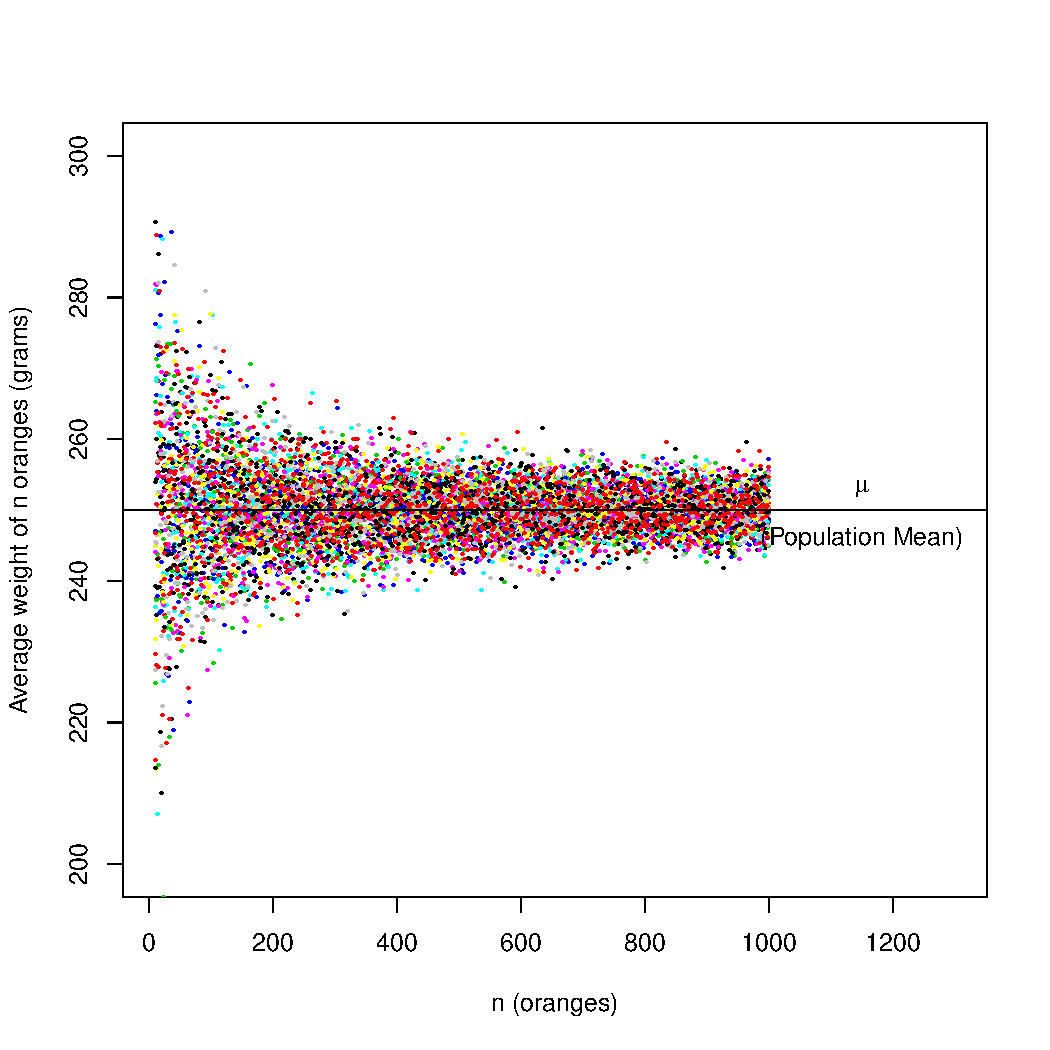
\includegraphics[width=\textwidth]{Statistics/multiple_trials}
  \caption{Demonstration of unbiasedness of $A_n$}
  \label{fig:multiple_trials}
\end{figure}
				
As for the second condition, $ \lim_{n\to\infty} \epsilon = 0 $, we need to first define the error: It is a distance metric between $A_n$ and $\mu$. Since $A_n$ itself is a random variable, a suitable distance metric is the probablistic variant of euclidean distance: \[d(A_n, \mu) = \sqrt{E[(A_n-\mu)^2]}\]. Since $E[A_n] = \mu$, this distance metric is nothing but the Standard Deviation of $A_n$! So, let us calculate the Standard Deviation of $A_n$:
	\begin{align*}
		Var[A_n] 	&= \frac{1}{n^2} * Var[X_1+X_2+....+X_n] \\
				&= \frac{1}{n^2} * E[(X_1+X_2+....+X_n)^2 - n\mu^2] \\
				&= \frac{1}{n^2} * E[nE[{X_k}^2] + n(n-1)\mu^2 - n\mu^2], \ k \in [1,n] \\
				&= \frac{\sigma^2}{n} \\
		\therefore,
		SD[A_n] 	&= \frac{\sigma}{\sqrt{n}}		
	\end{align*}

As $n$ increases, the Standard Deviation of $A_n$ decreases as $\sqrt{n}$. And, as $n$ approaches infinity, the Standard Deviation will approach zero. Figure \ref{fig:var_vs_n} shows how the spread of $A_n$ decreases with increasing $n$ value.
\begin{figure}
  \centering
    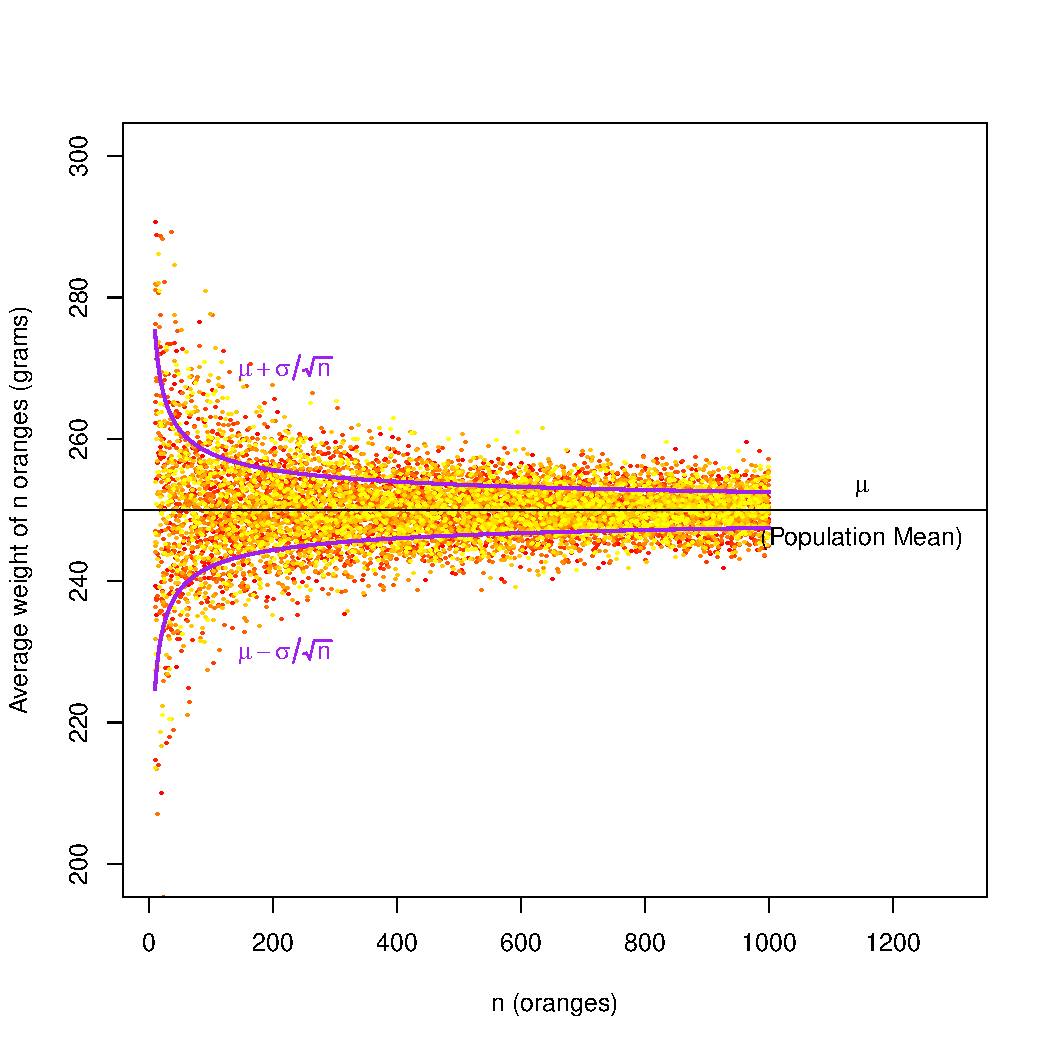
\includegraphics[width=\textwidth]{Statistics/var_vs_n}
  \caption{Reduction in the spread of $A_n$ values with increasing $n$}
  \label{fig:var_vs_n}
\end{figure}

\subsection{Law of Large Numbers}
We have established that the arithmetic average function is a good estimator of the population mean. But the arithmetic average of random variables itself is a random variable: Knowing its mean and Standard Deviation still doesn't guarantee that, if we conduct one trial and make one sample of $A_n$, it will not be wildly far away from the population mean. We won't be able to conduct several trials and come up with several samples of $A_n$ either: The very thing that got us think about finding an estimate for the population mean is that finding the exact population mean would require resources we cannot muster and gathering $n$ samples instead is affordable. If we can afford conduct serveral trials, then one might as well make an arithmetic average of all the samples of all the trials and call the new $n$ value as the total number of samples used for that average. In that case, we will be back starting at the fact that we have a single sample of $A_n$ and that could be widely far away from the population mean. But it would be such a shame if we can't say \emph{anything} about the size of the estimation error and, well, the field of statistics won't exist. This is where the law of large numbers comes into picture. There are two such laws, one called WLLN - the weak law of large numbers, and the other SLLN - the strong law of large numbers. The weak law states that the probability that the estimation error is greater than a certain bound will be lesser than a certain bound. And that, as $n$ becomes infinity, that probability will be zero. \\

	\begin{theo}[Weak law of large numbers]{thm:wlln} 
	\begin{align*}
	P(|A_n-\mu| > \xi) \leq \frac{\sigma^2}{n\xi^2} \\
	\therefore, \lim_{n\to\infty} P(|A_n-\mu| > \xi) = 0 
	\end{align*}
	\emph{where, $\xi$ is any arbitrary non-negative value}
	\end{theo}

The proof is simple: We expand the Variance formula for $A_n$ and segregate all items above $\xi$ as shown below:
	\begin{align*}
		Var[A_n] =  ...&+ \textcolor{blue}{(-\xi-\delta1)^2P(A_n-\mu = -\xi-\delta1) + (-\xi-\delta2)^2P(A_n-\mu = -\xi-\delta2) + ....}\\
				     &+ (-\xi)^2P(A_n-\mu = -\xi) \\
				     &+ (-\xi+\alpha1)^2P(A_n-\mu = -\xi+\alpha1) +  (-\xi+\alpha2)^2P(A_n-\mu = -\xi+\alpha2) + ....\\ 	
				     &+ (\xi)^2P(A_n-\mu = \xi) \\
				     &+ (\xi+\beta1)^2P(A_n-\mu = \xi+\beta1) +  (\xi+\beta2)^2P(A_n-\mu = -\xi+\beta2) + ....\\
				     &+\textcolor{blue}{(\xi+\eta1)^2P(A_n-\mu =\xi+\eta1) + (\xi+\eta2)^2P(A_n-\mu = \xi+\eta2) + ....}	
	\end{align*}
The terms in blue have probabilities of $|A_n-\mu| > \xi$. Noting that all probabilities are non-negative and the terms in front of the probabilities are also non-negative, the sum of all the terms in black will also be non-negative. Using this fact, and the fact that $Var[A_n] = \frac{\sigma^2}{n}$, we have,
	\begin{align*}
		 \frac{\sigma^2}{n} \geq  ...&+ \textcolor{blue}{(-\xi-\delta1)^2P(A_n-\mu = -\xi-\delta1) + (-\xi-\delta2)^2P(A_n-\mu = -\xi-\delta2) + ....}\\
				     			 &+\textcolor{blue}{(\xi+\eta1)^2P(A_n-\mu =\xi+\eta1) + (\xi+\eta2)^2P(A_n-\mu = \xi+\eta2) + ....}	
	\end{align*}
Now, using the same logic that we used to eliminate the terms that were black in colour, we have substitute $\xi$ in place of every term in front of the probabilities and we get, 
	\begin{align*}
		 \frac{\sigma^2}{n} \geq  ...&+ \textcolor{blue}{(\xi)^2P(A_n-\mu = -\xi-\delta1) + (\xi)^2P(A_n-\mu = -\xi-\delta2) + ....}\\
				     			 &+\textcolor{blue}{(\xi)^2P(A_n-\mu =\xi+\eta1) + (\xi)^2P(A_n-\mu = \xi+\eta2) + ....}	
	\end{align*}
Notice how we have removed the minus signs in the first line of the equation above? Well, it is because all the terms are squares - So it doesn't matter. Bringing all the $\xi^2$ to the left hand side of the equation, we get,
	\begin{align*}
		 \frac{\sigma^2}{n\xi^2} \geq  ...&+ \textcolor{blue}{P(A_n-\mu = -\xi-\delta1) + P(A_n-\mu = -\xi-\delta2) + ....}\\
				     			 &+\textcolor{blue}{P(A_n-\mu =\xi+\eta1) +P(A_n-\mu = \xi+\eta2) + ....}	
	\end{align*}	
The terms on the right side of the equation, when added together, essentially boil down to $P(|An-\mu| > \xi)$. Hence we get,
	\begin{align*}
		 \frac{\sigma^2}{n\xi^2} \geq  P(|A_n-\mu| > \xi)	
	\end{align*}
Since Standard Deviation of $A_n$ is  $\frac{\sigma}{\sqrt{n}}$, we can also rewrite the equation as,
	\[ P(|A_n-\mu| > \xi) \leq \frac{SD[A_n]^2}{\xi^2} \]
	
From the WLLN, we see that, knowing the number of samples and population variance, we could express our confidence that our estimate of the population mean is \emph{probably} accurate. In other words, we are quantifying our confidence. Just as Information Theory quantified information and built several useful constructs on top of that, Statistics builds many useful constructs based on the idea that confidence, and indirectly, chaos, can be quantified. In the next sections, we formally describe various methods in Statistical analysis for estimating population unknowns (\textbf{Estimation}), validating our assumptions about the population (\textbf{Hypothesis Testing}) etc. 

Note that, so far, we have only assumed that $X_1, X_2, ...., X_n$ are independent. When we formally introduce Estimation Theory, we can see that, depending upon how much more we know about these random variables (such as their probability distribution), we can get much tighter bounds on the error. 

\section{Estimation}
The population distribution and its parameters (mean, median, variance etc.) are all facts. There is no concept of likelihood associated with them. So the population is not a random variable and each possibility just has a frequency associated with it, and not a ``probability''. However, when you draw a random sample, $X_1, X_2, ...., X_n$, each $X_k$ is a random variable. And each $X_i$ has a probability distribution the same as the frequency distribution of the population, with the relative frequency as the probability \footnote{In fact, one way of looking at probability is that it is the relative frequency of a sample as the sample size approaches infinity, or, in our case, the size of the population}. The reason of this is that the $X_i$s are just placeholders for the $i$th draw and hence the probabilities of drawing a certain values is same as the relative frequency of it in the population. \textbf{Bear in mind, though, that this is true, strictly, only when we put back a drawn sample member back into the population before the next draw}. This is an important concept. Because if we don't put back what we drew from the population, the relative frequencies of all events/measurements/samples change because now there is one less member in that population. For, ex., suppose we are trying to estimate the mean weight of an orange in a crate, after randomly taking one orange and measuring its weight, we should put it back into the crate and draw the next random orange. 

The reality is a little bit different though. Often once we take one member out of the population, we don't put it back. Take the case of estimating the height of ten year olds in the state of Tamil Nadu - We will proceed by first choosing a sample size (which will depend upon our budget and other practical considerations \footnote{After all, Statistics is all about what is practically possible}). Let us say, that we decide on a sample size of 50. We are then likely to randomly select 50 ten year olds, measure their heights and call it our sample. This goes against the idea of putting back a selected individual back into the population before we select the next individual. But this is considered fine, as often, the population is very large compared to the sample size, and not putting back an ten year old into a population of 10 million ten year olds in Tamil Nadu, doesn't significantly alter the probabilities of any individual ten year old in the population from being selected in the next draw. Some Statisticians are OK with not putting individuals back, as long as the sample size is less than 1\% of the population. Some are even OK with it when the sample size is less than 10\% of the population. It is really up to the researcher at the end how much of an approximation error in the estimate is OK. 

\subsection{Maximum Likelihood Estimation}
One way to find an appropriate estimator for a population parameter, say $\theta$, for a given distribution, is to look at the random sample $X_1, X_2,...., X_n$ and ask, ``what $\theta$ value increases the joint probability of getting $X_1, X_2, ...., X_n$?''. In other words, suppose we define a function, $L(\theta)$ as,
	\[ L(\theta) = f(x_1;\theta).f(x_2;\theta)....f(x_n;\theta) = \prod_{i=1}^{n} f(x_i;\theta) \]
then, then $\theta$ value that maximizes $L(\theta)$ is the \textbf{Maximum Likelihood Estimate} (MLE) $\hat{\theta}$ of $\theta$. $L(\theta)$ is called the \emph{likelihood function}.

Let us take the example of estimating a population proportion. The measurements $X_i$s in this case, will (logically) follow a Bernoulli distribution. In other words,
	\[ f(x_i;p) = p^{x_i}(1-p)^{1-x_i} \]
So the likelihood function is,
	\[ L(p) = \prod_{i=1}^{n} p^{x_i}(1-p)^{1-x_i} = p^{\Sigma x_i}(1-p)^{n - \Sigma x_i} \]
To find the $p$ that maximizes $L(p)$, we have first take the derivative of $L(p)$ with respect to $p$ and equate it to zero, i.e., 
	\[ \frac{\mathrm d}{\mathrm d p} (p^{\Sigma x_i}(1-p)^{n - \Sigma x_i}) = 0 \]
Differentiating this is difficult. But we can use a neat trick: Since the likelihood function is a product of several probability values, it will always be a non-negative value. And we know that the logarithm function $log(\alpha)$ is an increasing function of $\alpha$. So taking the derivative of the logarithm of $L(p)$ and equating it to 0 will have the same effect of taking the derivative of $L(p)$ and equating it to 0. So, we have,
	\[ \frac{\mathrm d}{\mathrm d p} log (p^{\Sigma x_i}(1-p)^{n - \Sigma x_i}) = 0 \]
This, after some more derivation will yield,
	\begin{align*}
		 \Sigma x_i (1 - p) - (n - \Sigma x_i)p = 0 \\
		 \Sigma x_i - np = 0 \\
		 p = \frac{\Sigma x_i}{n}
	\end{align*}
To ensure that this extrema is actually the maxima, we need to take double derivative of $L(p)$ and evaluate it at $p = \frac{\Sigma x_i}{n}$ and make sure it is indeed a negative value. That is beyond the scope of this notes. Assuming that this is indeed the maxima, all we have to do now, to state the MLE for $p$, is use the random variable $X_i$ in place of the sample $x_i$ in the above result:
	\[\hat{p}_{MLE} = \frac{\Sigma X_i}{n} \]

In the case of proportions, we defined the likelihood function in terms of one parameter, $p$. But it can be generalized to multiple parameters as,
	\[ L(\theta_1,\theta_2,\ldots,\theta_m)=\prod\limits_{i=1}^n f(x_i;\theta_1,\theta_2,\ldots,\theta_m) \]
Let us look at an example where we derive the Maximum Likelihood Estimate of the mean and the variance of a Normally distributed population, from a random sample. The likelihood function in this case is:
	\[ L(\mu,\sigma)=\sigma^{-n}(2\pi)^{-n/2}\text{exp}\left[-\dfrac{1}{2\sigma^2}\sum\limits_{i=1}^n(x_i-\mu)^2\right] \]
As usual, we will take the log of the likelihood function before we move on to finding the extremas. But before that, for notational convenience, let us rewrite the likelihood function with generic parameters $\theta_1$ and $\theta_2$, in the place of $\mu$ and $\sigma^2$ respectively:
	\[ L(\theta_1,\theta_2)= \theta^{-n/2}_2(2\pi)^{-n/2}\text{exp}\left[-\dfrac{1}{2\theta_2}\sum\limits_{i=1}^n(x_i-\theta_1)^2\right] \]
Now we take the log of the likelihood function:
	\[\text{log} L(\theta_1,\theta_2)=-\dfrac{n}{2}\text{log}\theta_2-\dfrac{n}{2}\text{log}(2\pi)-\dfrac{\sum(x_i-\theta_1)^2}{2\theta_2} \]
Since we have two parameters, we need to do partial differentiations in order to find the extremas of the likelihood function with respect to one parameter at a time. First we do it for $\theta_1$:
	\[ \frac{\partial}{\partial \theta_1} L(\theta_1, \theta_2) = \frac{-2\Sigma(x_i - \theta_1)(-1)}{2\theta_2}  = 0\]
Resolving the equation, we get the estimate for $\theta_1$ as,
	\[ \hat{\theta}_1=\hat{\mu}=\dfrac{\sum x_i}{n}=\bar{x} \]

Now, doing the same for $\theta_2$, we get,
	\[ \frac{\partial}{\partial \theta_2} L(\theta_1, \theta_2) = \frac{-n}{2\theta_2} + \frac{\Sigma (x_i - \theta_1)^2}{2\theta_2^2} = 0\]
Multiplying both sides of the above equation by \( 2\theta_2^2 \) and solving for $\theta_2$, we get,
	\[ -n\theta_2 + \sum (x_i - \theta_1)^2 = 0 \]
	\[ \hat{\theta}_2 = \hat{\sigma}^2=\dfrac{\sum(x_i-\bar{x})^2}{n} \] 

Again, taking the second partial derivatives to confirm that the extremas are indeed maximas are beyond the scope of this notes. Assuming that this are indeed the maximas, all we have to do now, to state the MLE for the mean and the variance, is by using the random variable $X_i$ in place of the sample $x_i$ in the above results:
	\[ \hat{\mu}_{MLE} = \dfrac{\sum X_i}{n}=\bar{X} \]
	\[ \hat{\sigma}^2_{MLE} = \dfrac{\sum(X_i-\bar{X})^2}{n} \] 
	

\subsection{Method of Moments}
The method of moments involves equating sample moments with theoretical moments. So, let's start with their definitions \\
	
	\begin{defs}[Moments]{def:moments}
		\[ E(X^k) \text{is the $k$th theoretical moment about the origin} \]
		\[ E\left[(X-\mu)^k\right] \text{is the $k$th theoretical moment about the mean} \]
		\[ M_k=\dfrac{1}{n}\sum\limits_{i=1}^n X_i^k \text{is the $k$th sample moment about the origin} \]
		\[ M_k^\ast =\dfrac{1}{n}\sum\limits_{i=1}^n (X_i-\bar{X})^k \text{is the $k$th sample moment about the mean} \]
	\end {defs}
	
The idea of the method of moments is that, we create as many simultaneous equations as there are parameters to be estimated, by equating sample moments to theoretical moments. One can use moments about the origin or about the mean or a combination of both. For Bernoulli distribution's $p$ or Normal distribution's $\mu$ and $\sigma$, the \textbf{Method of Moments Estimate} (MM) ends up being trivial, as the paramters to be estimated themselves are theoretical moments - so we just use their sample moment equivalent as their corresponding estimates. But, let us look at the example of a Gamma distribution,
	\[ f(x_i)=\dfrac{1}{\Gamma(\alpha) \theta^\alpha}x^{\alpha-1}e^{-x/\theta} \] 
Here, the parameters $\alpha$ and $\theta$ are not the moments of the Gamma distributions. We use the MM Estimate for $\alpha$, $\theta$ as shown below:
	\begin{align*}
		E(X)=\alpha\theta=\dfrac{1}{n}\sum\limits_{i=1}^n X_i=\bar{X} \\
		Var(X)=\alpha\theta^2=\dfrac{1}{n}\sum\limits_{i=1}^n (X_i-\bar{X})^2 \\
		\intertext{From the first equation, we get $\alpha$ in terms of $\theta$:} 
		\alpha=\dfrac{\bar{X}}{\theta} \\
		\intertext{We substitute this in the second equation and get,} 
		\alpha\theta^2=\left(\dfrac{\bar{X}}{\theta}\right)\theta^2=\bar{X}\theta=\dfrac{1}{n}\sum\limits_{i=1}^n (X_i-\bar{X})^2 \\
		\intertext{Now, we can solve for $\theta$ and then use it to calculate $\alpha$ :} 
		\hat{\theta}_{MM}=\dfrac{1}{n\bar{X}}\sum\limits_{i=1}^n (X_i-\bar{X})^2 \\
		\hat{\alpha}_{MM}=\dfrac{\bar{X}}{\hat{\theta}_{MM}}=\dfrac{\bar{X}}{(1/n\bar{X})\sum\limits_{i=1}^n (X_i-\bar{X})^2}=\dfrac{n\bar{X}^2}{\sum\limits_{i=1}^n (X_i-\bar{X})^2}
	\end{align*}
	
\subsection {Unbiased Estimate}
We have so far seen two ways of coming up with estimates for distribution parameters. There may be even more ways of coming up with estimates. We need a way to evaluate how good these estimates are before we use them. One criterion is whether or not they are unbiased estimates. 
	\begin{defs}
		An estimate, \( \hat{\theta} \) is said to be \textbf{Unbiased Estimate} of the parameter \( \theta \) if:
		\[ E[\hat{\theta}] = \theta \]
	\end{defs}
	
For example, let us look at the MLE for the variance of the normal distribution:
	\[ \hat{\sigma}^2_{MLE}=\left(\dfrac{1}{n}\sum\limits_{i=1}^nX_i^2\right)-\bar{X}^2 \]
Taking the expectation of this Estimate, we get:
	\begin{align*}
		E(\hat{\sigma}^2_{MLE}) &= E\left[\dfrac{1}{n}\sum\limits_{i=1}^nX_i^2-\bar{X}^2\right]=\left[\dfrac{1}{n}\sum\limits_{i=1}^nE(X_i^2)\right]-E(\bar{X}^2) \\
		&= \dfrac{1}{n}\sum\limits_{i=1}^n(\sigma^2+\mu^2)-\left(\dfrac{\sigma^2}{n}+\mu^2\right) \\
		&= \dfrac{1}{n}(n\sigma^2+n\mu^2)-\dfrac{\sigma^2}{n}-\mu^2 \\
		&= \sigma^2-\dfrac{\sigma^2}{n}=\dfrac{n\sigma^2-\sigma^2}{n}=\dfrac{(n-1)\sigma^2}{n}
	\end{align*}

Since it doesn't meet the criterion, the MLE for the variance of the normal distribution is \emph{not} an unbiased estimate. So, what do we do now? Well, we can simply massage the last equation above as:
	\[ \dfrac{n}{n-1} E(\hat{\sigma}^2_{MLE}) = \sigma^2 \]
	\[ E( \dfrac{n}{n-1} \hat{\sigma}^2_{MLE}) = \sigma^2 \]
In other words, we can get the unbiased estimate of variance by multiplying the MLE for variance with $\frac{n}{n-1}$. This will result in:
	\[ \hat{\sigma}^2 = \dfrac{\left(\sum\limits_{i=1}^nX_i - \bar{X}\right)^2}{n-1} \]
	
	

\subsection {Estimating Mean When Variance is Known}
Suppose we are interested in estimating the mean of a population which is Normally distributed, where we know the Variance. This happens in situations where we are manufacturing, say resistors, and the machine used already has a known error spread. 

We already know that the sample average is a good estimate (It is the MLE, MM and unbiased estimate of $\mu$ 
 	\[ \bar{X} = \frac{\sum X_i}{n} \]
While we know that $\bar{X}$ is a good estimate of $\mu$, we also know that there will be some error in the estimation. WLLN gives us a way of quantifying the error with quantifying our level of confidence in that error. We recall it below for convenience:
	\[ P(|\bar{x}-\mu| > \xi) \leq \frac{\sigma^2}{n\xi^2} \]
Now when we derived WLLN, we mentioned how, knowing more information about the $X_i$ values could give us tighter confidence bounds on the error. So let us see what all we know in this situation.

It is a fair assumption that the $X_i$ are themselves Normally distributed with mean $\mu$ and variance $\sigma^2$. They are also independent of one another. We know that the sum of two Normally distributed, independent, random variables, will result in a Normally distributed random variable, with mean and variance equal to the sum of the means and sum of the variances of those two random variables ( \href{https://en.wikipedia.org/wiki/Sum_of_normally_distributed_random_variables}{Proof}  using convolution property). We also know any linear transformation of a Normal R.V. will result in a Normal R.V. (see \href{https://www.probabilitycourse.com/chapter4/4_2_3_normal.php}{proof})\footnote{The trick to deriving the pdf of a transformation of a continuous R.V. is through the CDF route - This is because, one will have to calculate the probability of the transformed variable, and for a continuous R.V. probabilities have to be derived from the CDF, as the probability of continuous R.V. to have an exact value is zero}. So, considering these facts, we can say that $\bar{X}$ will also be a Normal random variable. And we also know how to calculate its mean and variance. Here it is:
	\[ \bar{X} \sim \mathcal{N}(\mu,\sigma^2/n) \]

Knowing this, instead of an upper bound on the error, we can actually find the exact probability, \( P(|\bar{X}-\mu| > \xi) \) - In Estimation Theory, the actual practice is to instead find \( P(|\bar{X}-\mu| \leq \xi) \), which basically conveys the same meaning. Let us call this probibility value \(p_v\). We can derive \(p_v\) from the probability density funciton of \(\bar{X}\):
	\[ p_v = P(|\bar{X}-\mu| \leq \xi)  = P(\mu-\xi \leq \bar{X} \leq \mu+\xi) =   \int_{\mu-\xi}^{\mu+\xi}  \frac{1}{\sqrt{2\pi}(\sigma/\sqrt{n})} e^{-\frac{1}{2}\left(\frac{\bar{x} - \mu}{\sigma/\sqrt{n}}\right)^2} \mathrm{d}\bar{x} \]
Note that, 
	\[ P(|\bar{X}-\mu| \leq \xi) =  P(|\mu-\bar{X}| \leq \xi) \]. 
This also means, 
	\[ P(\mu-\xi \leq \bar{X} \leq \mu+\xi) = P(\bar{X}-\xi \leq \mu \leq \bar{X}+\xi) \]
In other words, the result of that integral can be interpreted as the probability that a calculated sample mean value $\bar{x}$ is within a certain distance from the population mean, or as the probability that the population mean $\mu$ is within a certain distance from the sample mean value $\bar{x}$. The latter statement is considered somewhat sacrilegious by statisticians, because they think no one should be making probability statement about a fact - i.e., here, the population mean. But nevertheless, this equivalence concept is handy because, what we know is $\bar{x}$, so it makes sense to say that we are certain cofident with a certain probability that $\mu$ lies within a certain distance of $\bar{x}$. In other words, instead of thinking of the distribution of the random variable $\bar{X}$ as a Normal distribution with population $\mu$ at its centre, we can think of the distribution of population $\mu$ with $\bar{x}$ (current sample mean, not the R.V), at the centre. Although $\mu$ is a constant, when it comes to the probability of the error, these two scenarios are equivalent. 

Anyway, once we calculate \(p_v\) from that integral, suppose it is say, 0.75, then we can make a statement, that, \emph{``we are confident that, 75 out of 100 times we conduct a trial (observe a \(\bar{X}\) value), the population mean will be within \(\pm \xi\) of the observed value of \(\bar{X}\)''}. Or as statisticians prefer to say, \emph{``we are 75\% confident that the population mean will be within \(\pm \xi\) of the observed value of \(\bar{X}\)''}. 

There is however one big problem: It turns out that the integral for calculating \(p_v\) is a pain in the posterior to evaluate analytically. So one has to use numerical methods to find out the result. If we are gong to calculate numerically, then it made sense that we do the exercise of calculating the integral for various limit values once and store the results in a lookup table - The next time we need to do this integral we could just look up the result on this table. But, unfortunately, this doesn't solve the problem either: The lookup table thus calculated would contain \(p_v\)s for one specific Gaussian - with one specific mean and standard deviation. If we never want to calculate the integral, then we would have to create one look up table for every possible value of mean and standard deviation. This is impossible! Enter the \textbf{Z statistic}:

We know that a linear transformation of a Normally distributed R.V. results in another Normally distributed R.V. Suppose we have an R.V. \(X \sim \mathcal{N}(\mu,\sigma^2)\), then we can derive another R.V.  such that it has a mean of \(0\) and a standard deviation of \(1\). Let us call this new R.V., \(Z\). The transform for calculating \(Z\) from \(X\) is as below:
	\[ Z = \frac{X-\mu}{\sigma} \mid Z \sim \mathcal{N}(0,1) \]
\(Z\) is called the \textbf{Standard Normal distribution}

In our case, since the random variable we are concerned with is \(\bar{X}\), we can derive \( Z = \frac{X-\mu}{\sigma/\sqrt{n}} \mid Z \sim \mathcal{N}(0,1) \). When we do this, we can translate \( P(\bar{X}-\xi \leq \mu \leq \bar{X}+\xi) \) into a probabilty on \(Z\) lying between new limits - let us call them, \( (-z_{\alpha/2}, z_{\alpha/2}) \) - such that:
	\[\arraycolsep=1.4pt\def\arraystretch{2.2}
	\begin{array}{rcccl} 
	-z_{\alpha/2} & \leq & \dfrac{\bar{X}-\mu}{\sigma/\sqrt{n}} & \leq & z_{\alpha/2}\\ 
	-z_{\alpha/2}\left(\dfrac{\sigma}{\sqrt{n}}\right) & \leq & \bar{X}-\mu & \leq & +z_{\alpha/2}\left(\dfrac{\sigma}{\sqrt{n}}\right)\\ 
	-\bar{X}-z_{\alpha/2}\left(\dfrac{\sigma}{\sqrt{n}}\right) & \leq & -\mu & \leq & -\bar{X}+z_{\alpha/2}\left(\dfrac{\sigma}{\sqrt{n}}\right)\\ 
	\bar{X}-z_{\alpha/2}\left(\dfrac{\sigma}{\sqrt{n}}\right) & \leq & \mu &\leq & \bar{X}+z_{\alpha/2}\left(\dfrac{\sigma}{\sqrt{n}}\right) 
	\end{array}
	\]
	
Now, we originally set out to find \( P(\bar{X}-\xi \leq \mu \leq \bar{X}+\xi) \) - If we compare this with the above inequality, if we set 
	\[ z_{\alpha/2} = \xi \dfrac{\sigma}{\sqrt{n}} \]
then, 
	\[ P(\bar{X}-\xi \leq \mu \leq \bar{X}+\xi) \equiv P(-z_{\alpha/2} \leq \dfrac{\bar{X}-\mu}{\sigma/\sqrt{n}} \leq z_{\alpha/2}) = P(-z_{\alpha/2} \leq Z \leq z_{\alpha/2}) \]
So we could create just one lookup table, called \textbf{Z table}, that has \( P(-z_{\alpha/2} \leq Z \leq z_{\alpha/2}) \) values calculated for various \( z_{\alpha/2} \) (at some granularity) and then use this table to calculate  \( P(\bar{X}-\xi \leq \mu \leq \bar{X}+\xi) \) using the above relationship. 
	
A note: The terminology of \( z_{\alpha/2} \) is not coincidental. It is common among Statisticians to refer to the Z value above which area under the pdf, i.e., probability, is \( \alpha/2 \) as \( z_{\alpha/2} \). So if we look at the probability between \( -z_{\alpha/2} \) and \( z_{\alpha/2} \), it will be \( 1 - \alpha \). i.e.,
One typical way statisticians ask about our confidence on our estimate \(\bar{X}\), is \emph{``What is your 90\% confidence interval?''}. Then one would translate it to an \(\alpha\) of 10\%, look up on the Z-table what \(-z_{0.05}, z_{0.05}\), and finally come with the answer as, \( \bar{X}-z_{0.05}\left(\dfrac{\sigma}{\sqrt{n}}\right),  \bar{X}+z_{0.05}\left(\dfrac{\sigma}{\sqrt{n}}\right) \).
	\[ \int_{-z_{\alpha/2}}^{z_{\alpha/2}}  \frac{1}{\sqrt{2\pi}} e^{-\frac{1}{2}z^2} \mathrm{d}z  = (1-\alpha)\]
Actually the normal practice among Statisticians, when it comes to estimation theory is not to start with an error threshold value and then answer the question of how confident we are that our estimation error is within that threshold value\footnote{In Hypothesis Testing, they use both ways}. Instead they define a \textbf{Confidence Interval}  \( [-z_{\alpha/2}, z_{\alpha/2}] \), such that,
	
When we are using the Z-statistic, the \( (1-\alpha)\% \) Confidence Interval on $\bar{x}$, i.e.,  \( [ \bar{x} - z_{\alpha/2}\left(\dfrac{\sigma}{\sqrt{n}}\right),\ \bar{x} + z_{\alpha/2}\left(\dfrac{\sigma}{\sqrt{n}}\right) ] \).  is called the \textbf{z-interval for the mean}. The most often used confidence intervals are 68\%, 95\% and 99.7\%, because these correspond to $z_{\alpha/2}$ values of 1, 2 and 3 respectively, or euivalently the error being one, two, three sampling standard deviations away, respectively. The standard deviation (or its estimate) of a sampling distribution is called the \textbf{standard error}\footnote{In the \emph{Probability Overview} section, when we talked about Variance, we discussed the idea of standard error}. 

Remember that z-interval works only if the samples are Normally distributed. What if they follow some other distribution? One way to tackle it is by using a large sample size $n$, due to Central Limit Theorem, $\bar{X}$ would look close to a Normal distribution. Then we can go ahead and use the z-interval. Of course, one could instead derive, from scratch, the appropriate test for a sample that doesn't have Normally distributed random variables, but that would also involve deriving area under the curve of whatever is the distribution of $\bar{X}$ - Most statistical softwares have tools for calculating z-interval. So, it is better to use, instead, a large $n$ and take advantage of tools in statistical softwares.
 
 
\subsection {Estimating Mean When Variance is Unknown}
 In most cases of social studies, we don't know the mean and the variance. To estimate the mean in this situation, we cannot use Z-table on the R.V., \(  Z = \frac{\bar{X}-\mu}{\sigma/\sqrt{n}} \). The logical thing to do is to substitute $\sigma$ with Sample Standard Deviation, $S$, where,
 	\[ S=\sqrt{\dfrac{1}{n-1}\sum\limits_{i=1}^n (X_i-\bar{X})^2} \].
But when we substitute \(S\), which is a Chi-squared distribution, in place of \(\sigma\) in \( \frac{\bar{X}-\mu}{\sigma/\sqrt{n}} \) the result will no longer be a Gaussian. It will instead be a Student's T distribution with $n-1$ degrees of freedom:
	\[ T=\dfrac{\bar{X}-\mu}{S/\sqrt{n}} \sim T(n-1) \]
The complete proof can be found \href{https://online.stat.psu.edu/stat415/lesson/2/2.5}{here}., but the basic idea is to recognize that:
	\begin{itemize}
	\item \(  Z = \frac{\bar{X}-\mu}{\sigma/\sqrt{n}} \sim \mathcal{N}(0,1) \)
	\item \( \dfrac{(n-1)S^2}{\sigma^2}\sim \chi^2_{n-1} \)
	\item \(\bar{X}\) and \(S^2\) are independent
	\end{itemize}

Anyways, instead of the confidence interval derived based on $z_{\alpha/2}$, we derive the interval based on the equivalent value on the \textbf{T-Table} called the \textbf{t-interval for mean}:
	\[ \bar{x}\pm t_{\alpha/2,n-1}\left(\dfrac{s}{\sqrt{n}}\right) \]
	
Note that, due to the Central Limit Theorem, as $n$ becomes large, the difference between z-interval and t-interval shrinks. Figure \ref{fig:T-Z-distributions} shows how, as the sample size increases, the t-distribution approaches the Z-distribution. When $n=30$, there is hardly any difference between the two distributions. So, some statisticians use the \(z_{\alpha/2}\) in place of \(  t_{\alpha/2,n-1} \) in the above equation for the t-interval,  if the sample size is greater than 30 \footnote{In general, the z-interval is tighter than a t-interval as the t-distribution would always have fatter tails than the Z-distribution. So a z-interval will be an underestimation of the estimation error in cases where t-inveral should have been used}. It is not fully clear why they would do that. It may have had some significance before the advent of computers when statisticians where using physical z-table, t-table charts - It is possible that carrying a single page of z-table is more convenient than carrying an entire book of t-tables, as there is one t-table for every $n$. 
	\begin{figure}
	  \centering
	    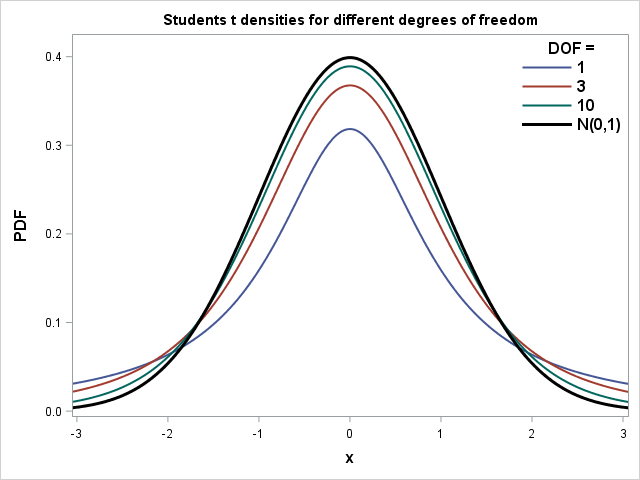
\includegraphics[width=\textwidth]{Statistics/T-Z-distributions}
	  \caption{T-distribution approaching Z-distribution as n increases}
	  \label{fig:T-Z-distributions}
	\end{figure}
	
\subsection {Estimating Difference in Means}
Quite often, we come across a situation, where we are interested in estimating the difference between two populations: For instance, the difference in response times between sobre and drunk people, the difference between the growth levels of the same species of plants under two different lighting conditions (with all else being equal) etc. In such situations, we can derive confidence intervals for \( \mu_X - \mu_Y \), where $X$ and $Y$ are used to describe the two different populations. We won't do the derivations here. One can find them in academic literature such as \href{https://online.stat.psu.edu/stat414/node/200/}{this} one. We will simply mention the intervals in Appendix \nameref{apdx:stat-at-a-glance}. But we will describe here when to use which of the different tests when it comes to confidence intervals for differences between means. In all cases, the populations are assumed to be Normally distributed.

We start with the simplest case where we know that the variance of both populations $X$ and $Y$ are the same and are known to us. And if we derive two random samples from $X$ and $Y$, with sample sizes $n$ and $m$ respectively, then,
	\[ \bar{X}-\bar{Y} \sim \mathcal{N}\left(\mu_X - \mu_Y, \frac{\sigma^2}{n} + \frac{\sigma^2}{m}\right) \]
We can call \( \bar{X} - \bar{Y} \) as $\bar{D}$, with \( \mu_D = \mu_X - \mu_Y \) and \( \sigma^2_D = \left(\frac{\sigma^2}{n} + \frac{\sigma^2}{m}\right) \). Then it is a case of a simple z-interval for a Normally distributed random variable as before:
	\[ \bar{d} \pm z_{\alpha/2}*\sigma_D \]

Th next case is when $X$ and $Y$ are considered to have the same variance, but that variance is unknown. So we need to instead use an unbiased estimate of this unknown variance. It turns out, ``pooled sample variance'', $S^2_P$ is an unbiased estimate of the population variance:
	\[ S_P^2=\dfrac{(n-1)S^2_X+(m-1)S^2_Y}{n+m-2} \]
And, with this, we can come up with a \textbf{Pooled t-interval} for difference between means. $\mu_X-\mu_Y$ as: 
	\[ (\bar{X}-\bar{Y})\pm (t_{\alpha/2,n+m-2}) S_P \sqrt{\dfrac{1}{n}+\dfrac{1}{m}} \]

But what if we know that $X$ and $Y$ have different variances and they are unknown? Then we have to use a \textbf{Welch's t-interval} as:
	\[ \bar{X}-\bar{Y}\pm t_{\alpha/2,r}\sqrt{\dfrac{s^2_X}{n}+\dfrac{s^2_Y}{m}} \]
where, $r$ degrees of freedom is approximated by:
	\[ r=\dfrac{\left(\dfrac{s^2_X}{n}+\dfrac{s^2_Y}{m}\right)^2}{\dfrac{(s^2_X/n)^2}{n-1}+\dfrac{(s^2_Y/m)^2}{m-1}} \]

The general practice is to use the Welch's t-interval when \(\dfrac{s^2_X}{s^2_Y} > 4\), or when \(\dfrac{s^2_Y}{s^2_X} > 4\). Otherwise, Pooled t-interval is used.

There is one more interesting case left, which is when, we are interested in estimating the mean of the differences, instead of the differences of means. As an example, suppose we are interested in knowing the effect of a certain fertilizer on the yield of many types of vegetable plants: Here it doesn't make sense to take a random sample from a group of vegetables where the fertilizer was not used (say, $Y$) and another from a group where the fertilizer was used (say, $X$). This is because, there may already be inherent differences in yields between different vegetables. So, for instance, if a tomato plant, under any condition, is expected to give more fruits per plant, than a brinjal plant under the same condition, then it doesn't make sense to take a random sample where there may be 5 tomato plants and 3 brinjal plants in the group of vegetables where the fertilizer wasn't used and 2 tomato plants and 6 brinjal plants in the group of vegetables where the fertilizer was used. Instead it may make sense to pair plants - For every measurement $X_i$, we measure a $Y_i$ where both measurements are taken from the same plant type. That way, we can literally compare ``apples to apples''. So in this case, we find the differences between paired measurements, i.e., \( D_i = X_i - Y_i \) and then estimate the mean of $D$, the population difference. We can come up with a \textbf{Paired t-interval} for $\mu_D$ as:
	\[ \bar{d} \pm t_{\alpha/2,n-1}\left(\dfrac{s_d}{\sqrt{n}}\right) \]
There are many instances when both $X_i$ and $Y_i$ are the same person in an experiment: Some examples are, the weight of persons before and after a diet regime, the effect of a medicine on sugar levels of diabetic persons etc. In all these cases, the above Paired t-interval is used.

\subsection {Confidence Intervals for Variances}
Estimation of variance is very important in manufacturing. Most goods manufactured are spec'ed out both for their nominal values (1/4'' screw, 3.3K Ohm resistor etc.), as well as their tolerances often specified as $pm x\%$. If the sample measurements are normally distributed, then, \textbf{\((1-\alpha)\%\) confidernce intervals for variance and standard deviation} are:
	\[ \left(\dfrac{(n-1)}{\chi^2_{\alpha/2,n-1}} S^2 \leq \sigma^2 \leq S^2\dfrac{(n-1)}{\chi^2_{1-\alpha/2,n-1}}\right) \]
	\[ \left(\dfrac{\sqrt{(n-1)}}{\sqrt{\chi^2_{\alpha/2,n-1}}} S \leq \sigma \leq S \dfrac{\sqrt{(n-1)}}{\sqrt{\chi^2_{1-\alpha/2,n-1}}}\right) \]
We won't derive the proof here, but it starts with realising that, 
	\[ \frac{(n-1)S^2}{\sigma^2} \sim \chi^2_{n-1} \]
	
Sometimes we need to estimate the ratio of two variances. There is a reason why we want to estimate the ratio of variances as opposed to difference in variances (like we do for means): For example, if you are a shirt manufacturer manufacturing clothese for Chinese as well as Indians, the differences between the mean height of Chinese and the mean height of Indians will tell you how much more cloth will be used on an average to make a shirt for an Indian compared to that for a Chinese. But variance will tell you how many SKUs need to be made for Indians vs. Chinese. A ratio makes sense here, because suppose variance in the height of Indians is twice as much as that of Chinese, then \( \text{No. of SKUs for Indians} = \text{No. of SKUs for Chinese} * \frac{\sigma^2_Indians}{\sigma^2_Chinese} \). Another reason for using the ratio is that, one can make sense of the square root of estimated ratio of variances as an estimate of the ratio of stardard deviations - and standard deviations are important as they have the same unit of measure as the measured quantity. However we can't say much about the difference in standard deviations between populations by looking at the estimate of the difference in their variances. For these reason, you can see that, even while estimating one variance, we start off by looking at the ratio of unbiased estimate of the variance to the variance. 

To find the confidence interval for ratio of variances, we first start with the following Chi-squared distributions related to the population and sample variances of R.V.s \(X\) and \(Y\) in question:
	\[ \dfrac{(n-1)S^2_X}{\sigma^2_X}\sim \chi^2_{n-1}\) and \(\dfrac{(m-1)S^2_Y}{\sigma^2_Y}\sim \chi^2_{m-1} \]
Here n and m are the number of samples used for calculating sample variances of \(X\) and \(Y\) respectively. Then we observed that, when \(X\) and \(Y\) are independent, the following ratio is a F-distribution of \(m,n\) degrees of freedom:
	\[ \dfrac{\chi^2_{m-1}/(m-1)}{\chi^2_{n-1}/(n-1)} \sim F(m-1, n-1) \]  
i.e., 
	\[ F=\dfrac{\dfrac{(m-1)S^2_Y}{\sigma^2_Y}/(m-1)}{\dfrac{(n-1)S^2_X}{\sigma^2_X}/(n-1)}=\dfrac{\sigma^2_X}{\sigma^2_Y}\cdot \dfrac{S^2_Y}{S^2_X} \sim F(m-1,n-1) \]	
Therefore, the following probability statement holds:
	\[ P\left[F_{1-\frac{\alpha}{2}}(m-1,n-1) \leq \dfrac{\sigma^2_X}{\sigma^2_Y}\cdot \dfrac{S^2_Y}{S^2_X} \leq F_{\frac{\alpha}{2}}(m-1,n-1)\right]=1-\alpha \]
From this, we can device confidence interval for ratio of variances as:
 	\[ \left(\dfrac{1}{F_{\alpha/2}(n-1,m-1)} \dfrac{s^2_X}{s^2_Y} \leq \dfrac{\sigma^2_X}{\sigma^2_Y}\leq F_{\alpha/2}(m-1,n-1)\dfrac{s^2_X}{s^2_Y}\right) \]

\subsection{Confidence Intervals for Proportions}
If one were to draw a random sample from a population that has a Bernoulli distribution, and count the number of time one of the two possible values occurred (no. of males or no. of heads etc.), the resulting random variable will have, a Binomial distribution. So one can derive confidence intervals based on Binomial distribution PMF. However the PMF becomes difficult to calculate\footnote{It is a question of how much computational power one has} when the sample size increases. At the same time, the count also starts looking more and more like a Normal distribution. This is because, if one assigned a value of $1$ for the one of the two possible values and $0$ for the other, then \( X_1+X_2+...+Xn \) will result in a Normally distributed R.V. as the $X_i$s are independent and identitically distributed (C.L.T). And if we also realize that the sample proportion $ \hat{p} = \sum_{i=0}^{n}\frac{ X_i}{n} $ is also the sample mean. So taking these two facts together, if the sample size is large, one could use a z-interval for means as the confidence interval for proportions, i.e., 
	\[ \hat{p}\pm z_{\alpha/2}\sqrt{\dfrac{p(1-p)}{n}} \]
But the problem in the above interval is that it is unreasonable that we would know the population variance $ p(1-p) $ directly, not could we have found it from the value of $p$, the value of which is the very thing we are trying to estimate. And we cannot use a t-interval like we did while estimating the mean of a Normally distributed population with the help of the sample standard deviation: For a Normally distributed population, the sample standard deviation is Chi-square distributed and hence the t-statistic is T-distributed. But in our present case of Bernoulli distributed R.V.'s, the sample standard deviation won't be Chi-square distributed. So, what do we do now? Well, the logical thing to do is to simply substitute $p$ with $\hat{p}$, but keep using the z-interval: 
	\[ \hat{p}\pm z_{\alpha/2}\sqrt{\dfrac{\hat{p}(1-\hat{p})}{n}} \]
Of course, this is an approximation, but we can't do any better.

So, we have been assuming that, when we draw a sample member from the population, we put it back before we make the next draw. But we often take surveys with ``Yes'' or ``No'' answers, where there is no concept of putting back an earlier draw before the next draw. In that case, \( X_1+X_2+...+X_n \) will not be a Binomial distriution, as Binomial requires that we put back a sample before the next draw. It is still fine to use Binomial distribution (extended to Normal R.V) in many cases because the sample size is typically very small when compared with the size of the population. But what about finite populations? For ex., if we are surveying the number of people in a village who approve a recent panchayat decision. Suppose the population of the village is only 2000, and we want to take a quick survey of just 50 people, and from them, gauge the approval rating for the panchayat. In this case, we cannot use a binomial distribution. Instead, it would follow a hyper-geometric distribution, that has mean $np$ and variance \( np(1-p) \left(\dfrac{N - n}{N - 1}\right) \), where $N$ is the size of our finite population (in our example, $N = 2000$, $n = 50$). While we could derive a confidence interval based on the hyper-geometric PMF, it is cumbersome\footnote{Computation power is cheap now-a-days. So it may be possible to compute a confidence interval based on the hyper-geometric PMF}. And even though the $X_i$s aren't identitically distributed, (because of non-replacement,) the sample mean, \( \hat{p} = \dfrac{X_1+X_2+...+X_n}{n} \), still approaches a Normal distribution. So, it is a normal practice among statisticians to use a z-interval for $\hat{p}$:
	\[ \hat{p}\pm z_{\alpha/2}\sqrt{\dfrac{\hat{p}(1-\hat{p})}{n} . \dfrac{N-n}{N-1}} \]
Note how this is identical to the confidence interval for $\hat{p}$ when the population is large, except for a ``correction factor'' to account for the finite population size. As one can easily see, if $n<<N$, then \( \dfrac{N - n}{N - 1} \) will work out approximately to unity. In other words, when the population is very large compared to the sample size, there is no difference between the confidence interval for $\hat{p}$ with or without replacement.

The confidence intervals for two proportions can use pooled t-interval or Welch's t-interval in the exact same way as we did with means, using the same logic that $\hat{p}$ is normally distributed and is also an estimate of the population proportion. 

\subsection{Determining Sample Size}
If we are trying to unearth facts about the population from data that is already available, then we are constrained by the sample size of that data set. All confidence intervals we have calculated so far involve sample size - The smaller the $n$ values, the wider, or loser, the interval. What if we are proavtively going to make measurements of some quantity to estimate the population fact? Then we have control over the sample size - We can decide how much max error \( \xi = |\theta - \hat{\theta}| \) is acceptable. Mostly the sample size will be constrained by the cost of making measurements, such as the budget allocated for the effort in dollars, the time we have in our hands to make the measurements, the man-hours of effort we are willing to put in etc. Here we will see some nuances about determining the sample size for our choice of error. 

We start with the confidence interval for the mean. We will assume that the variance of the population is unknown. When we define the confidence interval with a certain $\alpha$ value, what we mean is, we are \( (1-\alpha)*100\% \) sure that,
	\[ \mu = \bar{x} \pm t_{\alpha/2,n-1}\left(\dfrac{s}{\sqrt{n}}\right) \]
So the upper bound of the error is,
	\[ \xi = |\mu - \bar{x}| = t_{\alpha/2,n-1} \left(\dfrac{s}{\sqrt{n}}\right) \]
If we rearrange this equation, we can come up with the formula for $n$:	
	\[ n = t_{\alpha/2,n-1}^2 \left(\dfrac{s^2}{\xi^2}\right) \]

There are a couple of problems in this formula though: The first is that the t-distribution on the right side depends on the very $n$ that we are trying to find using it! The second is that the sample standard deviation $s$ is not known before we have a sample! The first problem can be taken care of by substituting the t-distribution with the z-distribution, because, while the t-distribution changes with $n$, the standard normal doesn't. However, recall that the t-distribution always has fatter tails than z-distribution (as shown in Figure \ref{fig:T-Z-distributions}. This means that substituting \( t_{\alpha/2,n-1}^2 \) with \( z_{\alpha/2}^2 \) will result in a smaller $n$ that what is right value for that $\alpha$ . One way to take care of this is by simply ensuring that $n$ is greater than 30 - because as one can see from Figure \ref{fig:T-Z-distributions}, when $n=30$, already there is very little difference between a t-distribution and the standard normal. 

The problems with not knowing the sample standard deviation $s$ can be taken care of using several methods. One of them is to use a smaller pilot survey/measurements and then using the $s$ from that sample to find the $n$ value for the actual survey/measurements. Another method is to use $s$ from a different study which involved taking sample from the same population as the one we are interested in. Yet another method is to judge the minimum and maximum values of the measurements and then use them as the end points of a 95\% confidence interval, and then, using \( s = \dfrac{Max-Min}{4} \), because a 95\% confidence interval is $\pm 2\sigma$ on either side of the mean. An example case where this is possible, is when we are trying to find out, say, the number of cups of tea drunk by Indians: We know that the minimum number of cups will be 0. And we personally may have never come across a person who drinks more than 10 cups of tea a day. If we are 95\% confident about this fact, then we can use $s = 2.5$ for estimating the sample size.

Determining the sample size required in the case of proportions of a large population, is very similar: We just substitute $s^2$ with \( \hat{p}(1-\hat{p}) \) in the last equation. However, calculating the sample size required for a finite population, when we don't replace draws, requires us to deal with the confidence interval we derived for this case earlier:
	\[ \hat{p}\pm z_{\alpha/2}\sqrt{\dfrac{\hat{p}(1-\hat{p})}{n} . \dfrac{N-n}{N-1}} \]
It can shown easily that this will result in the sample size equation:
	\[ n=\dfrac{m}{1+\dfrac{m-1}{N}} \]
where, $N$ is the size of the finite population and $m$ is sample size \emph{if} we were dealing with a large population, i.e:
	\[ m=\dfrac{z^2_{\alpha/2}\hat{p}(1-\hat{p})}{\xi^2}\]
This is like we calculate the sample size as if we are doing it for a large population (or for a small population, but with replacement), but then we account for a correction factor of \( 1+\dfrac{m-1}{N} \). As expected, this correction factor will work out to unity when $N$ is very large, and we will get $n=m$.

\section{References}
[1] \href{https://online.stat.psu.edu/stat414/}{PSU STAT 414: Introduction to Probability Theory}
[2] \href{https://online.stat.psu.edu/stat415/}{PSU STAT 415: Introduction to Mathematical Statistics}


